\documentclass{article}
\usepackage{amsmath}
\usepackage{amssymb}
\usepackage{amsthm}
\usepackage{graphicx} % Required for inserting images
\usepackage[margin=0.7in]{geometry} % Adjusted margins for better readability
\usepackage{enumitem} % Improved formatting for lists
%\usepackage{xcolor} % Required for defining colors
\usepackage{mdframed} % Required for framing the NOTE sections
\usepackage[usenames,dvipsnames,svgnames,table]{xcolor}
\usepackage{hyperref}
\hypersetup{
     colorlinks   = true,
     citecolor    = gray
}

\usepackage{tocloft}

\renewcommand{\cftsubsecfont}{\normalfont\hypersetup{linkcolor=purple}}
\renewcommand{\cftsubsecafterpnum}{\hypersetup{linkcolor=blue}}

% Define a color for the box
\definecolor{lightblue}{RGB}{173, 216, 230}

% Define a framed box for notes
\mdfdefinestyle{MyFrame}{%
    backgroundcolor=lightblue,
    roundcorner=5pt,
    frametitlerule=true,
    frametitlebackgroundcolor=white,
    frametitlerulecolor=lightblue,
    innertopmargin=\topskip,
}

\definecolor{lightorangered}{RGB}{255, 200, 173}

% Define a framed box for notes
\mdfdefinestyle{HW}{%
    backgroundcolor=lightorangered,
    roundcorner=5pt,
    frametitlerule=true,
    frametitlebackgroundcolor=white,
    frametitlerulecolor=lightblue,
    innertopmargin=\topskip,
}

% Define a color for the box
\definecolor{lightblue}{RGB}{173, 216, 230}

% Define a framed box for notes
\mdfdefinestyle{MyFrame}{%
    backgroundcolor=lightblue,
    roundcorner=5pt,
    frametitlerule=true,
    frametitlebackgroundcolor=white,
    frametitlerulecolor=lightblue,
    innertopmargin=\topskip,
}
% Define a framed box for notes
\mdfdefinestyle{MyFrame}{%
    backgroundcolor=lightblue,
    roundcorner=5pt,
    frametitlerule=true,
    frametitlebackgroundcolor=white,
    frametitlerulecolor=lightblue,
    innertopmargin=\topskip,
}
%permuatation and comb
\newcommand*{\permcomb}[4][0mu]{{{}^{#3}\mkern#1#2_{#4}}}
\newcommand*{\perm}[1][-3mu]{\permcomb[#1]{P}}
\newcommand*{\comb}[1][-1mu]{\permcomb[#1]{C}}
% Define a box for class session dates
\usepackage[most]{tcolorbox}

\NewTColorBox{classsessionbox}{O{}}{
    colback=white,
    colframe=lightblue,
    arc=0pt,
    outer arc=0pt,
    leftrule=0pt,
    rightrule=0pt,
    toprule=0pt,
    bottomrule=0pt,
    boxrule=0pt,
    right=0pt,
    top=5pt,
    bottom=5pt,
    width=3cm, % Set the width as needed
    title={\textbf{#1}},
    fontupper=\small, % Adjust the font size as needed
    halign=flush right, % Align to the right
}


\makeindex

% Define a theorem style
\theoremstyle{definition}
\newtheorem{theorem}{Theorem}
\usepackage{mathtools}
\DeclarePairedDelimiter\ceil{\lceil}{\rceil}
\DeclarePairedDelimiter\floor{\lfloor}{\rfloor}

\title{Probability(MA2202) Assignment 02 Solutions}
\author{Shuvam Banerji Seal (22MS076)\\ \small sbs22ms076@iiserkol.ac.in \\ GROUP - C}
%\date{January 2024}
\date{\today} % Adjusted to include the current date

\begin{document}

\maketitle
%\tableofcontents

\section{Problem 01:}
\begin{mdframed}[style = MyFrame]
\subsection{Problem Statement}
    There are $n$ boxes numbered $1,2,\ldots,n$, among which the $r$th box contains $r - 1$ white cubes and $n - r$ red cubes. Suppose, we choose a box at random and we remove two cubes from it, one after another, without replacement.

(a) Find the probability of the second cube being red.

(b) Find the probability of the second cube being red, given that the first cube is red.
\end{mdframed}

\subsection{Solution:}
\textbf{Part : a}\\
    Let $P(r)$ be the probability of choosing rth box.\\
    $P({w_1}_r)$ = $P({w_1}|r)$ be the probability that the 1st ball is white given that the rth box is chosen.\\
    $P({R_1}_r)$ = $P({R_1}|r)$ denotes the probability that 1st ball is red.\\
    $P({R_2}_r|{R_1}_r)$ denotes the probability that second ball is red given that from the rth box, the 1st ball chosen is red.\\
    $P({R_2}_r | {w_1}_r)$ denotes the probability that the second ball is red given that the first ball chosen from the rth box is white.\\
    Now, 
    \[
    P(R_2) = P(1). P({R_2}_1) + P(2). P({R_2}_2) + \dots + P(n-3). P({R_2}_{n-1}) + P(n-2). P({R_2}_{n-2}) + P(n-1). P({R_2}_{n-1}) + P(n). P({R_2}_{n})   
    \]
    \[
    = \frac{1}{n} \cdot ( P({R_2}_1) + \dots + P({R_2}_{n-2}) + P({R_2}_{n-1}) + P({R_2}_{n})
    \]
    \[
    = \frac{1}{n} \cdot ( \sum^{n} (P({w_1}_r). P({R_2}_r | {w_1}_r) + P({R_1}_r). P({R_2}_r | {R_1}_r))
    \] \[
     = \frac{1}{n} \cdot ( \sum_{r=1}^{n} (\frac{(n-r)(r-1)}{(n-1)(n-2)} + \frac{(n-r)}{n-1}\cdot \frac{n-r-1}{n-2}))
    \]
    \[
    =   \frac{1}{n} \cdot ( \sum_{r=1}^{n} (\frac{(n-r)(r-1+n-r-1)}{(n-1)(n-2)}))
    \]
    \[
    =   \frac{1}{n} \cdot ( \sum_{r=1}^{n} (\frac{(n-r)(n-2)}{(n-1)(n-2)}))
    \]
    \[
    = \frac{1}{n(n-1)} \cdot ( \sum_{r=1}^{n} (n-r))
    \]
    \[
    = \frac{n(n-1)}{2} \cdot \frac{1}{n(n-1)}
    \]
    \[
    = \frac{1}{2}
    \]
\\
\textbf{Part: b}\\
Now, the probability of having the 2nd ball being red, when it is given that the first ball is red, is calculated as the following:
\[
P(R_2|R_1) = \sum_{r=1}^{n-1} P(r) \cdot P({r_2}_r|{R_1}_r)
\]
as the nth box has no red balls, so $P({R_1}_r) = 0$
\[
    = \frac{\sum_{r=1}^{n} (\frac{n-r}{n-1}) \cdot (\frac{n-r-1}{n-2}) \cdot \frac{1}{n}}{\frac{1}{2}}
\]

\[
 = \frac{2}{n(n-1)(n-2)} \cdot \sum_{r=1}^{n}  (n-r)({n-r-1})
\]

\[
= \frac{2}{n(n-1)(n-2)} \cdot \sum_{r=1}^{n}  [(n-r)^2-({n-r})]
\]

\[
= \frac{2}{n(n-1)(n-2)} \cdot [\frac{n(n-1)(2n-1)}{6} - \frac{n(n-1)}{2}]
\]

\[
= \frac{1}{(n-2)} \cdot  [\frac{2n-1}{3} - 1]
\]

\[
= \frac{1}{(n-2)} \cdot \frac{2n-4}{3}
\]
\[
= \frac{2}{3}
\]
So, the second ball being red given that the first ball is from the rth box is $\frac{2}{3}$

\vspace{0.5cm}
\section{Problem 02:}
\begin{mdframed}[style = MyFrame]
\subsection{Problem Statement}
Let $(\Omega, \mathcal{E}, P)$ be a probability space and let $A_1, A_2, \ldots, A_n \in \mathcal{E}$ with $P(A_1 \cap \ldots \cap A_n) \neq 0$. Show that 
\[ P(A_1 \cap \ldots \cap A_n) = P(A_1)P(A_2|A_1)P(A_3|A_2\cap A_1)\ldots P(A_n|A_{n-1}\cap\ldots\cap A_1).  \]
\end{mdframed}

\subsection{Solution:}
\begin{proof}
 Given, $P(A_1 \cap \ldots \cap A_n) \neq 0$, so $\frac{1}{P(A_1 \cap A_2)}$, $\frac{1}{P(A_1 \cap A_2 \cap A_3)}$, $\dots$, $\frac{1}{P(A_1 \cap A_2 \cap \dots \cap A_n)}$, is well defined. (As neither o the denominators are 0).\\
 So,
 \[
 P(A_1).P(A_2|A_1). P(A_3| A_2 \cap A_1). \dots P(A_n | A_1 \cap \dots \cap A_{n-1})
 \]
 \[
 = P(A_1) \cdot \frac{P(A_2 \cap A_1)}{P(A_1)} \cdot \frac{P(A_3 \cap A_2 \cap A_1)}{P(A_1 \cap A_2)} \dots \frac{P(A_{n} \cap \dots \cap A_1)}{P(A_{n-1} \cap \dots \cap A_1)}
 \]
 \[
 = P(A_{n} \cap \dots \cap A_1)
 \]

\end{proof}

\section{Problem 03:}


\begin{mdframed}[style = MyFrame]

\subsection{Problem Statement:}
Let $(\Omega, \mathcal{E}, P)$ be a probability space and let $A_1, A_2, \ldots , A_n$ be pairwise mutually exclusive. Let 
\[A = \bigcup_{n=1}^{\infty}A_n\] 
and let $B \in \mathcal{E}$ with $P(B) \neq 0$. Show that 
\[P(A|B) = \sum_{n=1}^{\infty} P(A_n|B).\]
\end{mdframed}
\subsection{Solution:}

\begin{proof}
  
    Let's start,
    \[
    P(A|B) = \frac{P(A \cap B)}{P(B)}
    \]
    \[
    = \frac{P(B \cap (A_1 \cup A_2 \cup \dots \cup A_n))}{P(B)}
    \]
    \[
    = \frac{P((B \cap A_1) \cup ( B \cap A_2) \cup \dots \cup (B \cap  A_n))}{P(B)}
    \]
    \[
    = \frac{P(A_1^w \cup A_2^w \cup \dots \cup A_n^w)}{P(B)} \quad \dots \text{ \quad Here} [A_i^w = (B \cap A_i), \text{which are disjoint.}]
    \]
    \[
    = \frac{\sum_{n=1}^{\infty} P(A_n^w)}{P(B)}
    \]
    $\because$ $A_n^w$'s are mutually exclusive, as for any $i,j \in \mathbb N$, $A_i^w \cap A_j^w = (B \cap A_i \cap A_j) \subseteq ( A_i \cap A_j) = \phi$, so any arbitrary number of intersections of $A_i$'s are $\phi$.
    \[
       = \frac{\sum_{n=1}^{\infty} P(A_n \cap B)}{P(B)}
    \]
\[
   = \sum_{n=1}^{\infty} P(A_n | B)
\]

\end{proof}

\section{Problem 04:}
\begin{mdframed}[style = MyFrame]
    \subsection{Problem Statement:}
    We are familiar with the famous Monty Hall problem. Now suppose, instead of 3 doors, there are $n$ doors, only one among which has a prize behind it.

(a) Find the probability of winning upon switching given that Monty opens $k$ doors. Will switching benefit you?

(b) Find the probability of winning upon switching given that Monty opens the maximum number of doors. Will switching benefit you?

(c) Find the probability of winning upon switching given that Monty opens no doors. Will switching benefit you?
\end{mdframed}
\subsection{Solution:}
\textbf{Part : A}\\
Let $P(A)$ denote the probability of prize being behind the 1st chosen door. Let $P(K)$ denote the probability of Monty opening $K$ doors, none of which has the prize behind them. So,
\[
P(A|K) = \frac{P(A).P(K|A)}{P(K)}
\]
Now, $P(K) =1$, as Monty knows which door does not have the prize. Similarly, $P(K|A) =1$
\[
\implies P(A|K) = P(A) = \frac{1}{n}
\]
\[
\implies P(A^c|K) = 1 - \frac{1}{n} = \frac{n-1}{n}
\]

But, here $P(A^c|K)$ denotes the probability that the prize is there in one of the $(n-1-k)$ doors, which are neither chosen  or opened, but those doors are indistinguishable (Of course). So, they would carry the same probability. The remaining doors which are not chosen and not opened will have $\frac{n-1}{n(n-k-1)}$ probability of having the prize. \\
Now, we have,
\[
P(A) = \frac{1}{n} < \frac{1}{n} \cdot \frac{n-1}{n-k-1}
\]
$\dots$ so, the above expression shows that \textbf{switching will be better.}

\textbf{Part : B}\\

Max no. of doors opening st the game can still go on is $n-2$.
Now putting $k=(n-2)$, in the expression from part A, we get the probability of closed or unchosen doors to contain the prize is $\frac{n-1}{n(n-1)(n-2)} = \frac{n-1}{n} > \frac{1}{n}$. \\
Here as well \textbf{switching will be better.}

\textbf{Part : C}\\
Again putting, $k=0$, in the expression from Part A, we get the probability of a closed or unchosen door to contain the prize is $\frac{n-1}{n(n-1)}=\frac{1}{n} = P(A)$, so \textbf{switching will be better.}
%\begin{comment}
\begin{figure}[h]
    \centering
    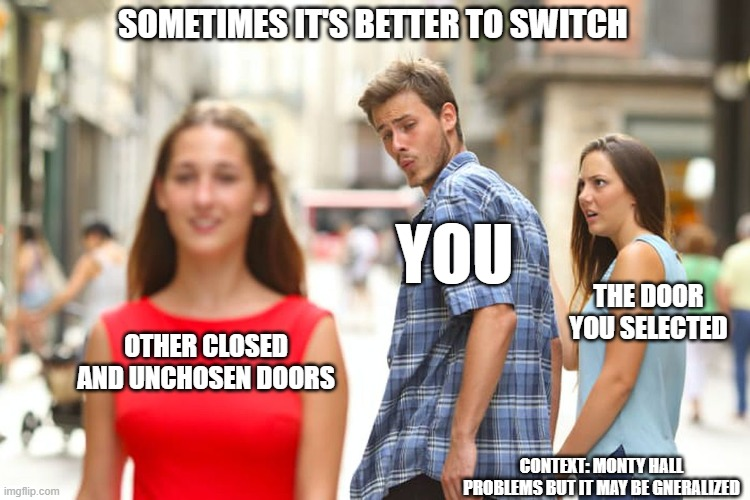
\includegraphics[scale = 0.27]{memem.png}
    \caption{Just a meme for this Monty hall stuff}
    \label{fig:enter-label}
\end{figure}
\section{Problem 05:}
\begin{mdframed}[style = MyFrame]
%\end{comment}
\subsection{Problem Statement:}

   Let \((\Omega, \mathcal{E}, P)\) be a probability space and let \(A_1, A_2, \ldots, A_n \in \mathcal{E}\) with \(P(A_1 \cap \ldots \cap A_n) \neq 0\). Show that 
\[ P(A_1 \cap \ldots \cap A_n) = P(A_1)P(A_2|A_1)P(A_3|A_2\cap A_1)\ldots P(A_n|A_{n-1}\cap\ldots\cap A_1).  \]

\end{mdframed}
\subsection{Solution:}
\begin{figure}[h]
    \centering
    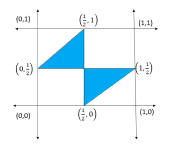
\includegraphics{sol5.png}
    \caption{Graphically depicting the Inequalities of the conditions}
    \label{fig:Illustration for sol 5}
\end{figure}

To form a triangle, it is necessary and sufficient condition that the sum of lengths of two-segment is greater than the third one.

If we take $x$ and $y$ are the ordinate and abscissas of two points chosen at random on the interval are $(0, 1)$.

The shaded can be represented using either of following inequalities.

\[ 0 < x < \frac{1}{2} < y < 1 \quad \text{and} \quad y - x < \frac{1}{2} \]

Or

\[ 0 < y < \frac{1}{2} < x < 1 \quad \text{and} \quad x - y < \frac{1}{2} \]

We know that area of triangle is given by $A = \frac{1}{2} \cdot b \cdot h$.

The probability of the shaded region is given as follows.

\[ P = \left( \frac{1}{2} \times \frac{1}{2} \times \frac{1}{2} \right) + \left( \frac{1}{2} \times \frac{1}{2} \times \frac{1}{2}   \right) \]

\[ \Rightarrow P =\left(   {\frac {1 } {8 }} + \frac{1}{8}   \right) \]



\[ \Rightarrow P= {\left(   {\frac {1 } {4 }}    \right)} \]


The probability that three-line segments form a triangle is
\[ P= {\left(   {\frac {   1 } {4 }}    \right)}. \]

\end{document}


